
{\chapter{Single  cell  whole genome fitness  landscapes  induced  by pharmacologic perturbations in cancer}
}
\label{ch:Chapter4}

\section{Motivation}
As discussed in introduction chapter 1, tumor fitness landscape underpin selection in cancer evolution and response to chemotherapy. However, quantifying clonal fitness in heterogeneous tumor populations remains an open problem that hampers effective treatment leading to tumor recurrence. Previous work has established models of fitness through interpreting allelic measurements of single snapshots \cite{williams2016identification, williams2018quantification,gerstung2020evolutionary,shah2012clonal,nik2012life} from bulk sequencing over large patient cohorts \cite{martincorena2017universal}, timeseries study of cell free DNA \cite{khan2018longitudinal}, multiregion sequencing \cite{Gerlinger2014-qd,Jamal-Hanjani2017-yc,Lopez2020-ku,mcpherson2016divergent,williams2018quantification} and estimating fitness landscapes of clonal haematopoiesis \cite{Watson2020-yu}. Moreover, the cancer field has generally lacked serial measurements from patient derived tissues to directly observe cancer evolution over realistic timescales. This has impeded a thorough understanding of causal factors driving selection, achieved in other biological systems through studying granular timeseries with population genetics modeling \cite{good2017dynamics}. Taking multiple measurements is critical for understanding  given behavior of cancer clones that are forced to evolve over time, and doing so at equal intervals give an open opportunity to clearly investigate the dynamics of that behavior manifesting at distinct time scales. Infact, patient derived xenograft (PDX)\cite{aparicio2015examining} systems are an effective model to study timeseries of a human tumour cell population \cite{williams2018using,willey2015patient}.
The majority of the work on cancer has focused on bulk tumour sequencing, where cellular population structure decomposition approaches are limited. Single cell genome measurements to scalably define clonal populations in cancer over thousands of cells have only recently emerged \cite{Laks2019-dm,zahn2017scalable}, enabling identification of rare populations, precise tracking of clones and robust clone-specific measurements suitable for population genetics modeling. We are also motivated by newly developed quantifying tools of \texttt{sitka}, a phylogenetic inference method accompanying toolkits to assign cells to clones, \cite{dorri2020efficient} and  \texttt{fitClone}, a probabilistic framework that designates quantitative selection coefficients to individual cancer clones and forecasts competitive clonal dynamics over time \cite{salehi2020single}. Motivated by these observations, we sought to investigate the hypothesis that clones that grow reproducibly have higher fitness in the growing cancer.



\section{Synopsis}
Based on the knowledge we gained from chapter 3 for transplant efficiency and initial tumor responses to chemotherapies, we selected four \textit{Tp53} mutant \ac{PDX} for this chapter \textbf{\autoref{tab:Tp53mutationofPDX}}. Three TNBC and one HER2+ \ac{PDX} tumors. For the chemotherapy, two drugs (cisplatin and CX-5461) were selected to investigate clonal dynamics and identify patterns of clonal resistance with single cell whole genome sequencing in treated and untreated timeseries. First we, studied un-treated 4 transplanted timeseries, including two PDXs (HER2+SA532 and TNBC-SA609), especially passaged upto ten generations(X1 to X10). By applying newly developed methods, for identifying sub-populations with their genotypes, 
e showed that serial measurements of single cell copy number assigned clones can be used to estimate fitness in conjunction with \texttt{fitClone} \cite{salehi2020single}. Under serial transplantation of breast patient derived xenografts, where no drug selection or other conditions were applied, we found that serial measurements can be used to measure relative clonal fitness which enables prediction of future trajectories.

Next, we sought to  confirm the reproducibility and independence of dynamics to population size effects, we re-ran the serial transplantation experiments after mixing early and late populations and re-measuring the dynamical behaviour. We observed that sufficiently well sampled clones with confident fitness estimations show repeated trajectories, confirming the estimation of fitness and linking the dynamical behaviour to the copy number genotypes of the clones.

Finally, we determined whether the fitness of clones under chemotherapy can be measured and asked whether clones exhibiting drug resistance are also fitter in the absence of selective pressure from chemotherapy. 

On all the single cell whole genome sequencing data, we applied three types of scientific computational methodologies. First, \textbf{sitka}, for computing phylogenetic trees and identifying genotypic clones, then using \textbf{Lumberjack} (a tree-cutting algorithm) and their relative abundances as a function of time. Last, \texttt{fitClone}, to measure the selection coefficient for each clone (\textit{s}) which we hypothesise to indicate growth potential. The larger the value of \textit{s}, the more fit the clone is relative to the chosen reference clone. 

%-----------------------------------------------------------

 % Table generated by Excel2LaTeX from sheet 'Tp53_PDX_mutation_small'
 \begin{table}[htbp]
   \centering
   \caption{\textit{Tp53} mutation status of all PDX}
     \begin{tabular}{|l|l|l|l|}
     \hline
     Sample ID & Protein Change & p53 Mutation Type & HGVSg \\
     \hline
    TNBC-SA1035  & C242F & Missense\_Mutation & 17:g.7577556C>A \\
     TNBC-SA609 & R213* & Nonsense\_Mutation & 17:g.7578212G>A \\
     HER2+SA532 & A159P & Missense\_Mutation & 17:g.7578455C>G \\
     TNBC-SA535 & V147Gfs*2 & Frame\_Shift\_Ins & 17:g.7578490\_7578489insC \\
     \hline
     \end{tabular}%
   \label{tab:Tp53mutationofPDX}%
 \end{table}%


%...........................................................
%% Figure 1 - schematic
\begin{figure}
\centering
\includegraphics[width=\textwidth]{Figures/chap4/fig1thesischap4.png}
\caption{Schematic overview of experimental design for quantitatively modeling clone-specific fitness.\textbf{a)} timeseries PDX systems All nodes representing each PDX tumour were digested to acquire genomes of single cells ($approx$200-600 cells/tumor). Extra replicate tumors at each time point are not shown in the diagram (n=2-4). Grey circles represent un-treated, blue represents Cisplatin treated and grey with a blue outline denotes drug-holiday samples \textbf{b)} Clonal dynamics of cell populations observed over time. Whole genome single cell sequencing of timeseries samples gives copy number (left) that in turn is used to infer a phylogenetic tree (middle), and clonal fractions over time (right) \textbf{c)} \texttt{fitClone}: mathematical modeling of fitness with diffusion approximation to the K-type Wright-Fisher model}.
\label{fig:schematic}
\end{figure}

%-------------------------------------------------------------


\section{Results}

\subsection{Modeling clonal fitness and selection}
With close collaboration of our bioinformatic colleagues, we  developed an experimental and computational platform consisting of three major components: scalable phylogenetics for single cell genomes to identify clones, timeseries sampling of patient derived xenografts over multiple month timeframes to observe clonal dynamics, and a mathematical model for inferring clone-specific fitness measures (\textbf{\autoref{fig:schematic}}). We studied breast cancer PDX, sequencing $>$123,106 cells over interval passaging (\textbf{\autoref{fig:schematic} a}), with single cell whole genome sequencing\cite{laks2019clonal} (scDNAseq, DLP+ method) from 101 libraries. From single cell copy number profiles we calculated phylogenetic trees to identify genotypic clones and their relative abundances as a function of time (\textbf{\autoref{fig:schematic} b}).
Timeseries clonal abundance observations were modeled using an implementation of the Wright-Fisher diffusion process  (\textbf{\autoref{fig:schematic} c}, we called \texttt{fitClone} \textbf{see methods}). \texttt{fitClone} simultaneously estimates growth trajectories, $X_i$ and fitness coefficients, $s_i$ for each clone $i$ in the population. 
We note that even small increments in $1+s_i$ indicate positive selection and higher growth potential. The model accounts for drift as well as selection, with fitness estimated relative to a reference population, where $s=0$ by construction. As a generative process, the model can be used for forecasting evolutionary trajectories of specific clones and posterior probability densities can be interpreted for evidence of positive selection in polyclonal systems. 

We carried out simulation experiments to establish theoretical behaviour and limitations of \texttt{fitClone}, over a range of parameters.  In two key advances, simultaneous modeling of multiple clones was superior to modeling each clone independently, and accounting for stochasticity in the dynamics via the diffusion process led to more accurate selection coefficient estimates than with a deterministic growth model (\textbf{\autoref{fig:simulations} a}). Model fits were robust to effective population size ($N_e$) and number of clones (\textbf{\autoref{fig:simulations}b,c}). Together these simulations established a rationale for systematic modeling of all clones in a unified approach, enabling  interpretations of dynamics exhibited in polyclonal cancers.

\subsection{Establishment of untreated timeseries patient derived xenografts}

To understand and quantify fitness attributes of cancer cells as  predictive measures of their growth potential in polyclonal systems, we set out to establish timeseries patient derived xenografts (PDX) with and without pharmacological perturbations (\textbf{\autoref{fig:schematic} a}).
Serial transplantations of four \textit{p53 mutant} human breast cancers were performed by injecting patient derived tumor cells and clumps into primary engrafted mice to secondary and subsequent recipients in a timeseries manner (\textbf{\autoref{fig:Untreatedgrowthcurves} a-top), n=3-4 at each time point)}. 
We generated timeseries observations from these untreated PDX, sampled over 927 days for HER2+SA532, 619 days for TNBC-SA609, 381 days for TNBC-SA1035 and 353 days for TNBC-SA535. 

To asses the growth potential over time and receptor status information, two PDXs (HER2+SA532 and TNBC-SA609-Line 1) were passaged comparatively longer, upto ten generations (X1-X10).
 (\textbf{\autoref{fig:Untreatedgrowthcurves} a-Bottom}).
 A median of 907 single cell genomes were sequenced per passage for a total of 11,705 and 10,553 single cell genomes from the HER2+SA532 and TNBC-SA609-Line 1 series, respectively. 
Growth record in all of timeseries exhibited progressively higher tumour growth rates over time (\textbf{\autoref{fig:Untreatedgrowthcurves} b}, \textbf{\autoref{fig:SA609allcyclescisplatin} b-d}). To confirm the architecture and integrity of patient's tumor, H \& E and immuno-histochemistry staining of paraffin embedded tumor sections were created at each time point with a set of standard markers. \textbf{(See Methods, {\autoref{fig:HistologyHER2+TNBC}} a, b)} is showing representative images of initial and late passages of tumor sections. 

%------------------------------------- 
 \begin{figure}
\centering
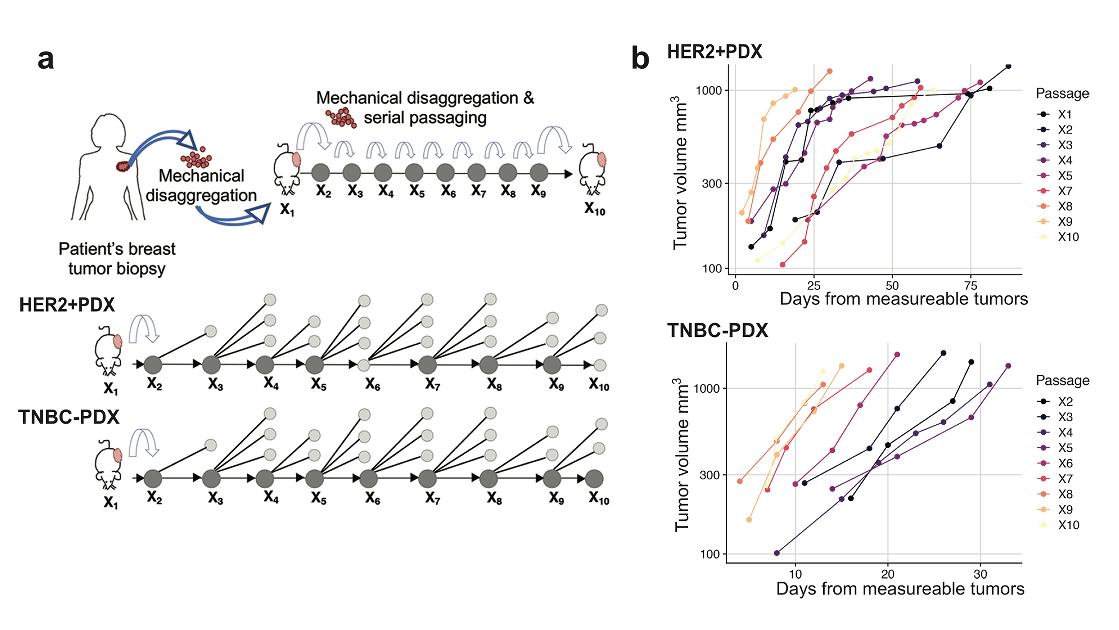
\includegraphics[width=\textwidth]{Figures/chap4/Untreatedgrowthcurves.png}
	
\caption[Untreated PDX timeseries and growth trajectories]
	{\small
	\textbf{Untreated PDX timeseries and growth trajectories.}
	    \textbf{(a)}, Top: Schematic for PDX timeseries; Bottom: Serial sampling of HER2+SA532 and TNBC-SA609 PDX tumours;
Dark grey circles represent each sampled mouse for scWGS. The light grey circles representing the replicates of tumour-bearing mice at the same timepoint. Small light grey at X6 and X10 represents absent data points.
	    \textbf{(b)}, Individual tumour growth from each passage of TNBC-SA609 and HER2+SA532 PDXs. Y-axis is showing the tumor volume in cubic millimeter while the x-axis is representing the time in days, tumors could be measured.}
	\label{fig:Untreatedgrowthcurves}
\end{figure}

%-----------------------------------------------------------

\begin{figure}
\centering
\includegraphics[width=\textwidth]{Figures/chap4/SA535_SA532.png}
	
\caption[Untreated PDX timeseries clonal dynamics at single cell level]
	{\small
	\textbf{Comparison of fitness landscapes of TNBC-SA535 and HER2+SA532 untreated breast cancer PDX timeseries models.}
	    \textbf{a)} Heatmap representation of copy number profiles of 1,549 cells, grouped in 10 phylogenetic clades. \textbf{b)} Phylogeny of cells over the timeseries TNBC-SA535 where nodes are groups of cells (scaled in size by number) with shared copy number genotype and edges represent distinct genomic breakpoints. \textbf{c)} Observed clonal fractions over time. \textbf{d)} Inferred trajectories and \textbf{e)} quantiles of the posterior distributions over selection coefficients of \texttt{fitClone} model fits to TNBC-SA535 with respect to the reference clone C. \textbf{f-j} Analogous to \textbf{a-e} but for HER2+SA532 (n=2,193 cells; reference clone A).}
\label{fig:SA535heatmapdynamicsHER2}
\end{figure}

%-----------------------------------------------------------
\subsection{Copy number associated clonal fitness in \textit{p53 mutant} human breast cancers}

Next, we sought to study clonal expansions through serial passaging, acquiring single cell whole genome sequencing and applying fitness modeling to all four \textit{p53 mutant} PDX timeseries.
DLP+ libraries were generated and sequenced, yielding a median of 303 single cell genomes per sample (9,970 total cells) of high quality for downstream analysis. Bulk WGS and DLP+ confirmed all four tumors harbored \textit{TP53} mutations (TNBC-SA609: \textit{p.R213X}; TNBC-SA1035: \textit{p.C242F}; HER2+SA532: \textit{p.A159P}; TNBC-SA535: \textit{p.V147Gfs*2}) with bi-allelic and truncal distribution across clones (\textbf{\autoref{tab:Tp53mutationofPDX}}).
Resulting phylogenetic analysis indicated all PDX were polyclonal at the copy number level.


%-------------------------------------------------------------

\begin{figure}
\centering
\includegraphics[width=\textwidth]{Figures/chap4/UnRxseries.png}
	
\caption[Untreated PDX timeseries clonal dynamics at single cell level]
	{\small
	\textbf{Comparison of fitness landscapes of two untreated breast cancer PDX timeseries models.}
	    \textbf{(a, b)} Clonal dynamics of TNBC-SA1035 and TNBC-SA609 models.
	    \textbf{(c)} Probability of positive selection in both PDX
	    \textbf{(d)} Heatmap representation of copy number profiles of 2,193 cells, grouped in 4 phylogenetic clades. 
	    \textbf{(e)} Phylogeny (simplified type II sitka tree) of cells over the timeseries TNBC-SA1035  Untreated PDX, where nodes are groups of cells (scaled in size by number) with shared copy number genotype and edges represent distinct genomic copy number change points (sitka markers)
 
\textbf{(f)} Top: growth trajectories, Bottom: Inferred \texttt{fitClone} trajectories
\textbf{(g)} selection coefficients for the HER2+ model. 
 \textbf{(h-k)} Analogous plots for the TNBC model (n=3,216 cells).
 
	}
	\label{fig:SA1035SA609UnRx}
\end{figure}
%-------------------------------------------------------------


\subsubsection{Phylogenetics and fitness analysis of untreated timeseries PDXs}
 For all timeseries, we inferred single cell copy number profiles , constructed a phylogenetic tree using \textbf{sitka} model taking copy number states as input to establish clonal lineages and measured clonal abundances as a function of time \textbf{(\autoref{fig:SA535heatmapdynamicsHER2} }, \textbf{\autoref{fig:SA1035SA609UnRx}}). For each timeseries (branch), we pulled all single cells to infer a phylogenetic tree \textbf{(See introduction and methods for details)}. The tree was cut using Lumberjack to yield clones and their abundances over time. Then \texttt{fitClone} inferred selection coefficient of a clone by reporting the posterior mean 1 + s followed by its standard deviation.

\subsubsection{Untreated timeseries HER2+SA532 PDX undergo neutral clonal dynamics as compared to TNBC-SA535}
In contrast with HER2+SA532, the TNBC PDX models exhibited evidence of clonal dynamics and variation in selection coefficients consistent with positive selection and differential fitness (\textbf{\autoref{fig:Mixturenew} a}). 
In TNBC-SA535, we acquired scWGS on 5 consecutively transplanted timepoints (X5, X6, X7, X8, X9) untreated \textbf{(\autoref{fig:schematic} a)} \textbf{(\autoref{fig:treatedtimeseriesmanuscript} b)} for a total of 1,341 single cells (mean = 335, $\sigma$ = 84.4 per timepoint).
11 clones \textbf{(\autoref{fig:SA535heatmapdynamicsHER2} a, b, c}) were observed, although only three major clones propagated after the initial time point.
The inferred clonal fractions were A(0.003), B(0.702), C(0.034), D(0.006), E(0.006), F(0.013), and G(0.237). Other 4 were below the threshold.
Clone C was chosen as the reference clone as it had a monotonically decreasing clonal fraction trajectory in the untreated branch. Clonal trajectories were consistent with selection coefficients
with small relative differences in fitness (\textbf{\autoref{fig:SA535heatmapdynamicsHER2} a-d}). Clone G had the highest fitness (1 + s = 1.01 $\pm$ 0.00751) \textbf{\autoref{fig:SA535heatmapdynamicsHER2} a-d}. 
 Clone G, characterized by \textbf{loss of ChrX} exhibited expansion from minor prevalence at passage X5 to near dominance at 76\% at passage X9 (selection coefficient $1+s$ = 1.02  $\pm$  0.01, (\textbf{\autoref{fig:SA535heatmapdynamicsHER2}}). 
 However, the HER2+SA532 series exhibited 4 distinct clones ranging in size from 134 to 1,421 cells ( \textbf{median 319, \textbf{\autoref{fig:SA535heatmapdynamicsHER2} e, f}}). Notably, none of the clones in the HER2+ series exhibited $1+s$ $>$ 1.015 suggesting a lack of positive selection.
 Clonal trajectories in the HER2+ model, were consistent with selective coefficients with small relative differences in fitness (\textbf{\autoref{fig:SA535heatmapdynamicsHER2} f-i})

\subsubsection{Untreated timeseries TNBC-SA1035 and TNBC-SA609 PDX undergo deterministic clonal dynamics}
For TNBC-SA1035, scWGS data collected from an untreated branch with five serial passages (X4, X5, X6, X7, and X8) \textbf{\autoref{fig:treatedtimeseriesmanuscript} b)} with a total of 2,015 single cells. 11 clones were detected (\textbf{\autoref{fig:SA1035SA609UnRx} a,b}) with clone E expanding to 69\% at passage X8 from minor prevalence at the initial timepoint (selection coefficient $1+s$ = 1.06 $\pm$0.03) (\textbf{\autoref{fig:SA1035SA609UnRx} c,d}). Clonal fractions over all timepoints in the untreated branch were A(0.097), B(0.140), C(0.087), D(0.160), E(0.266), F(0.010), G(0.058), H(0.053), I(0.065), J(0.018), and K(0.047). The reference clone A in this series had initial prevalence of 20\% but was not detectable by the last timepoint. Clone E rose from a clonal fraction of 0.028 at X4 to 0.69 at X8 and had the highest selection coefficient (1+s = 1.06 $\pm$ 0.0367). \textbf{Clone E} formed a distinct clade in the phylogeny, distinguished by a hemizygous deletion of the centromeric locus of \textbf{Chr8p}, an extra copy gain of the telomeric end of \textbf{Chr11q} and a focal gain of \textbf{Chr 9q21} harboring the \textit{CCNE1} locus as compared to reference clone C (\textbf{\autoref{fig:SA1035SA609UnRx} a}, \textbf{\autoref{fig:genotype609mix} a}).

Similarly, in untreated TNBC-SA609 timeseries, six clones were observed and clones E (\textbf{\autoref{fig:SA1035SA609UnRx} b}, light blue, $1+s$ = 1.07 $\pm$ 0.02 ) and H (\textbf{\autoref{fig:SA1035SA609UnRx}} b, light purple, $1+s$ = 1.02 $\pm$ 0.02) had the highest selection coefficients, exhibiting growth from undetectable levels to 59\% and 32\% respectively by timepoint X10. Clone C contracted from near 100\% at the initial timepoint to undetectable levels by X10 \textbf{\autoref{fig:SA1035SA609UnRx} g-i}). Growth of clones E, G, and H and contraction of clone C was observed reproducibly from replicate transplants (\textbf{\autoref{fig:genotype609mix} d}).
Consistent with increased dynamics in the TNBC-SA609 line 1 series, we found an initial increase of 0.1 breakpoints per cell per generation in the first 4 passages \textbf{(\autoref{fig:mutationanalysisbreakpoints} a)}. Clone E also had the highest number of breakpoints with 12.8 additional copy number breakpoints per cell, relative to the reference clone C with the lowest (linear regression with coverage breadth, ploidy and cell cycle state as covariates (p $<$0.0001) \textbf{(\autoref{fig:mutationanalysisbreakpoints} c)}.

By contrast, in all 3 TNBC series at least one clone showed a high degree of clonal fitness with pairwise probability of positive selection $>$ 0.9  \textbf{\autoref{fig:Mixturenew} a},\textbf{(\autoref{fig:landscapefitness} a}), consistent with diverse CNA clonal genotypes linked to high variation in fitness.

\subsection{Clone-specific fitness estimates forecast clonal competition trajectories} 
We next asked whether the high predicted fitness of Clone E was a true indicator of positive selection through a physical clonal mixing and re-transplant experiment. Enforced clonal competition of higher fitness clones with lower fitness counterparts should result in re-emergence or fixation of high fitness clones, even when re-starting from a low population prevalence. To test this, we performed mixture experiments by extracting cells from an early (X3) and a late (X8) passage of TNBC-SA609 (line 1) timeseries PDX and then physically mixed them. We established two such lines with different proportions \textbf{(also see methods)}.
In first \textbf{branch a}, we aimed to have a mixture comprising approximately of equal proportions from the two timepoints ($\approx$~50\% each) at the ratio of 1:1. In \textbf{branch b}, we aimed to have far less cells from late passage that contains the high fitness clone. The (71\% of X3 passage and 29.0\% of cells from the X8 passage) a ratio of 1:0.4.


\subsubsection{Clones with higher selection coefficients out compete low fitness clones in mixture branch a}
To validate the selection coefficients as indicators of positive selection, we forward-simulated trajectories from \texttt{fitClone} using estimated selection coefficients (B=1.00 $\pm$ 0.01, D=1.00 $\pm$ 0.01, G=1.01 $\pm$ 0.01, H=1.02 $\pm$ 0.02, E=1.07 $\pm$ 0.02). We compared two independent starting clonal proportions of (B=0.08, C=0.25, D=0.51, E=0.02, G=0.08, H=0.07) and (C=0.02, D=0.00, E=0.05, G=0.06, H=0.87), derived by mixing cells from a late (X8) and an early (X3) passage of the TNBC-SA609 (Line 1) series in mixture-retransplant-serial passage experiments as mentioned above \textbf{\autoref{fig:Mixturenew} b}). Simulated trajectories from the first set of starting proportions resulted in \textbf{clone E} with the highest probability of fixation (0.39). Fixation probabilities for the remainder of clones were low ($<$0.01). \textbf{\autoref{fig:Mixturenew} c} shows the simulated trajectories in black.
The mean clonal fraction at each step is shown in red. All clones except for clones E and H are predicted to vanish to clonal fractions of below 1\%. 

%We have combined the trajectories for clones E and F since clone F (i) had fewer than 19 total cells in the original series and consequently its selection coefficient had a high variance, (ii) is phylogenetically proximal to clone E \textbf{\autoref{fig:Mixturenew} d} and thus likely represented a biologically similar population and (iii) finally, is not observed above a threshold of 20 cells in any other line in the TNBC-SA609 family.

We experimentally tested these predictions by initiating a new PDX line with the remixed population (from M0), serially passaged over 4 timepoints \textbf{\autoref{fig:Mixturenew} b} (top), and sequenced with DLP+ (6,453 single cell genomes, median 1,287 per library). After placing the cells from all timepoints of this mixture experiment on the tree, they got assigned to six clones from the original timeseries were recovered having 26 to 767 (median 155) cells \textbf{\autoref{fig:Mixturenew} d-left} . In \textbf{\autoref{fig:Mixturenew} c} blue dots show the observed clonal fractions at each timepoint in PDX branch a. Clones with higher selection coefficients swept through the mixture timeseries by passage 4 (\textbf{\autoref{fig:Mixturenew} d-middle, right}). Comparison of model fits of the original and mixture timeseries yielded similar posterior distributions for the majority of clones. As anticipated by the model, clone E emerged as a high fitness clone ($1+s$ = 1.08  $\pm$ 0.03), and at the last timepoint, clones E and H comprised 94\% of cells \textbf{\autoref{fig:genotype609mix} c, d, e}. 
The estimated selection co-efficients were relatively strongly correlated (Pearson correlation of 0.795, considering only clones that reached overall prevalence of over 1\% in the original series.
%-------------------------------------------------------------

\begin{figure}
\centering
\includegraphics[width=\textwidth]{Figures/chap4/Mixturenew.png}
	
\caption[Reproducible dynamics from SA609-TNBC mixture experiments]
	{\small
	\textbf{Reproducible dynamics from SA609-TNBC mixture experiments}. In each panel, mixture a is followed by mixture b.
	    \textbf{(a)} Distribution over the probability of positive selection over pairs of clones computed as $\max(P(s_i > s_j), 1-P(s_i > s_j))$. The dots coloured purple denote probability of positive selection over 0.9.
	    \textbf{(b)} Clonal proportions of X3 and X8 used to generate the initial mixture M0 and subsequent serial passaging, yielding 4 samples M1-M4 for mixture a (top) and 5 samples M1-M5 for mixture b (bottom).
	    \textbf{c)} For mixture a: (left) Forward simulations using the median of inferred selection coefficients from the original timeseries and starting population proportions in the initial experimental mixture. Simulated trajectories are shown superimposed with median simulation (red line) and observed (blue dots); (middle) Inferred trajectories of mixture timeseries; (right) quantiles of the selection coefficients with respect to the reference clone C of \texttt{fitClone} fit to M1-M4 clonal abundance observations.
      \textbf{d)} Phylogenies showing cells observed in the mixture a (left), Inferred trajectories of mixture a timeseries (middle), Selection coefficients of \texttt{fitClone} fit to M1-M4 clonal abundance observations (right). \textbf{e} as in \textbf{d} but for mixture b (with respect to reference clone C).}    

	\label{fig:Mixturenew}
\end{figure}

%-----------------------------------------------------------
\begin{figure}
\centering
\includegraphics[width=\textwidth]{Figures/chap4/genePlotsa609mix.png}
	
\caption[Tumour evolution in absence of pharmacologic perturbation]
	{\small
	\textbf{Tumour evolution in absence of pharmacologic perturbation}
	    \textbf{a)} Copy number genotype of clone E and \textbf{b)} copy number genotype of clone C, the reference clone (arrows indicate differences to clone E).  
	    \textbf{c)} Evolution in absence of treatment and as a function of drug treatment. For each sample, the phylogeny with clonal abundance from DLP+ is shown, reflecting selection. \textbf{d)} The observed clonal abundances and \textbf{e)} the summarised clonal phylogenetic tree.}
	\label{fig:genotype609mix}
\end{figure}

%-------------------------------------------------------------------------

\subsubsection{Mixture branch b recapitulates the predicted dynamics of branch a and the original untreated branch}

Similar to mixture a, for mixture branch b (low proportion clone E mix), we initiated another new PDX, serially passaged over 5 timepoints \textbf{(\autoref{fig:Mixturenew} b}), and sequenced with DLP+  (6,730 single cell genomes, median 1,270 per library).
We forward simulated 10,000 trajectories using identical selection coefficient values as the first mixture branch a, but different clonal proportions, estimated from adding cells from timepoint X1 in mixture branch b to the TNBC-SA609 phylogenetic tree and assigning them to the corresponding clones (C = 0.02, D = 0.00, E = 0.05, F = 0.00, G = 0.06, H = 0.87). Unlike mixture branch a, DLP+ data was not available for timepoint M0 in mixture branch b.
For the second mixture \textbf{(\autoref{fig:Mixturenew} e}), cells from four clones (C, E, G, and H) from the original timeseries were observed (clone D had only  1 cell). Clone E was the only clone that increased in prevalence (from 5 to 24\%) and had the highest selection coefficient ($1 + s$ = 1.02 $\pm$ 0.03.  By contrast, Clones C, G and H appeared to exhibit neutral fitness. 

The analysis of the two mixture series suggests that (i) we can validate the selection coefficients estimated from a timeseries using \texttt{fitClone} and (ii) it is possible make quantitative predictions about the likely trajectories of tumour subpopulations at least at the clade level. Also, in the prediction trajectories plot \textbf{(\autoref{fig:Mixturenew} c, f)}, the time-axis for the observations is shrunk to best match the mean predicted trajectories line (red line). The diffusion time horizon that is obtained by dividing the generation time measured in days by the effective population size estimate results in trajectories that are ahead of the biological system.
Thus, both mixture experiments resulted in expansion of the highest fitness clone E, even when starting from proportions of 0.02 and 0.05, consistent with the predicted selection coefficients and forecasts of clonal competition.

%-------------------------------------------------------------
\begin{figure}
\centering
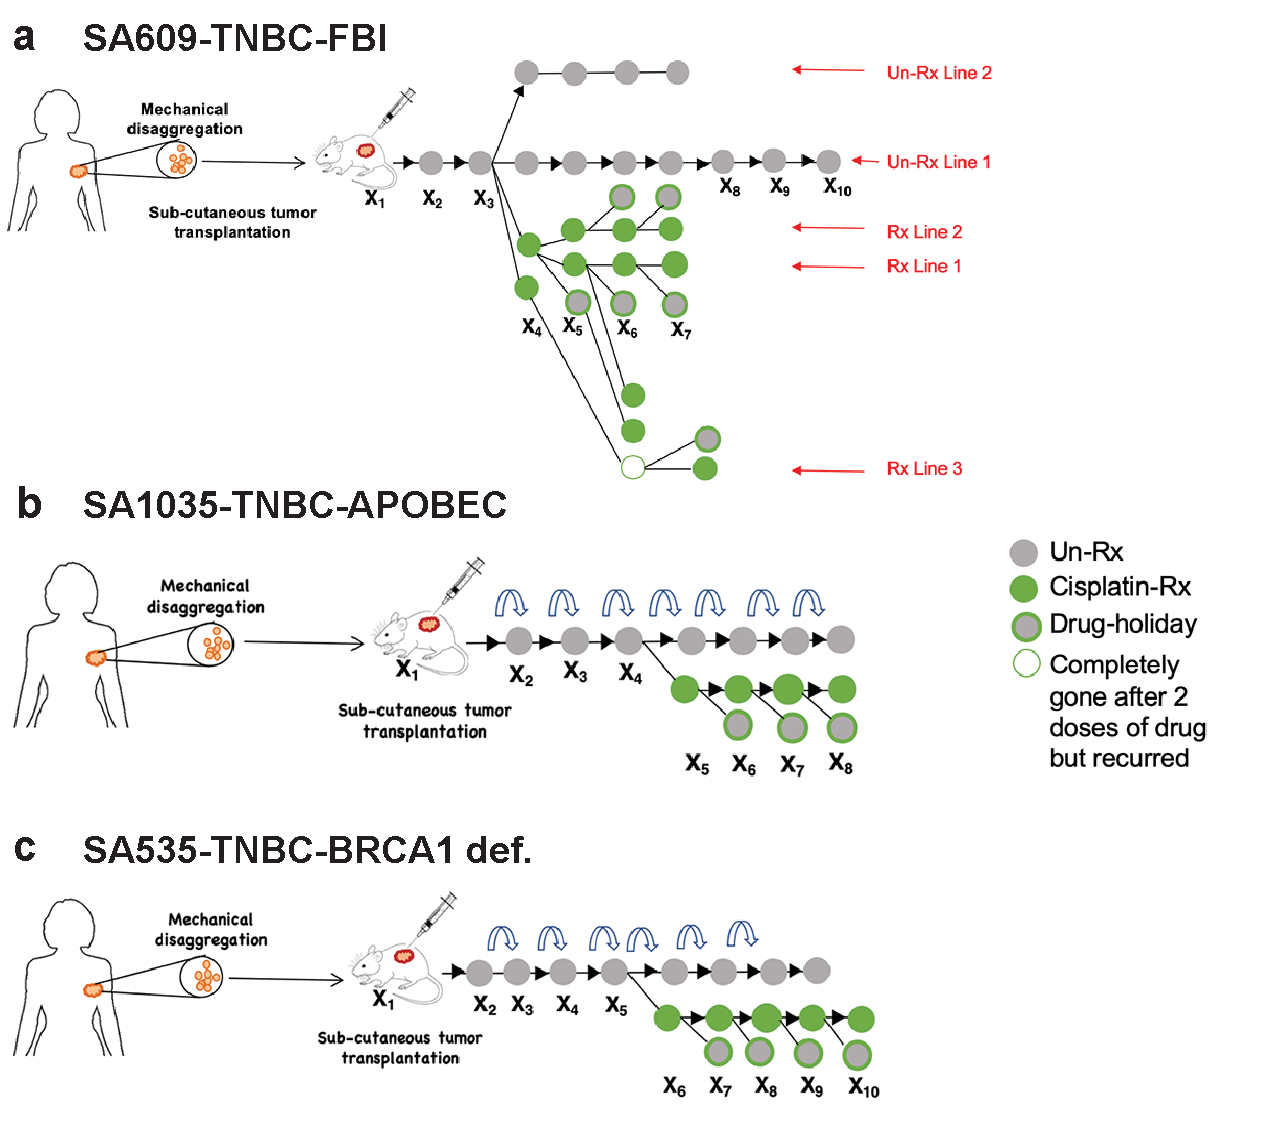
\includegraphics[width=\textwidth]{Figures/chap4/treatedtimeseriesgreen.pdf}

\caption[Experimental overview of TNBC PDX treated time series]
	{\small
	\textbf{Experimental overview of cisplatin treated TNBC PDX timeseries.}
	      All nodes representing each PDX tumour were digested to acquire genomes of single cells (~200-600 cells/tumor). Extra replicate tumors at each time point are not shown in the diagram (n=2-4). Grey circles represent un-treated, green represents Cisplatin treated and grey with green outline presents drug-holiday samples \textbf{(a)} SA609-TNBC time series with replicate treated and un-treated branches. DLP+ collected starting from X1 to X10 (Un-Rx line 1). Top grey branch indicating Un-Rx line 2. The middle three branches are cisplatin treated time series replicate branches \textbf{(b)} SA535-TNBC showing the tumor nodes taken for DLP+ starting from X5 untreated \textbf{(c)} SA1035-TNBC showing the tumor nodes taken for DLP+ starting from X 4 untreated.}
	
	\label{fig:treatedtimeseriesgreen}
\end{figure}

%...............................................................
\subsection{Clonal competition and fitness costs of platinum resistance}
So far, we have applied our framework to pharmacologically unperturbed tumor environment to track human cancer clones as identified by their Copy number genotypes over time and to reason about their likely abundances and validating them with specific experimental conditions. Next, we asked how drug treatment perturbs the fitness landscape. We investigated how cisplatin, an analog of platinum salts used as a standard therapy for primary TNBC, impacted the stability of the clonal dynamics in the three TNBC PDX (TNBC-SA609, TNBC-SA535, TNBC-SA1035).

%we investigate whether establishing baseline fitness measures could help to interpret selection under drug administration. We first present the TNBC-SA609 series in detail and make an observation about early response to cisplatin treatment. We then analyse two additional TNBC PDX lines to check the reproducibility  and generalizability of our observation.

\subsubsection{Repeated platinum exposure introduced drug resistance in \textit{p53 mutant} TNBC PDXs} 
 To test pharmacologic perturbation with cisplatin (platinum) impacted the stability of the fitness landscape of the TNBC series, we propagated a separate branch, for each of the series (\textbf{\autoref{fig:schematic} ,\autoref{fig:treatedtimeseriesgreen} a, b, c}). Cisplatin (2mg/kg) was administered once every 3 days for 8 doses maximum (Q3Dx8 max) through intraperitoneal (IP) injections, over at least four successive passages to induce drug resistance  (\textbf{\autoref{fig:SA609allcyclescisplatin}}, Supplementary  Information). Gradual onset of platinum resistance was physically confirmed with progressive reduction in tumour growth inhibition (TGI) \cite{hather2014growth} (\%TGI from first to last cycle: TNBC-SA609=77\%-4.7\%; TNBC-SA1035= 76\%-15\%; TNBC-SA535= 58\%-16\%, \textbf{\autoref{fig:SA609allcyclescisplatin}} b-d).
 
 For each serially treated tumour, a parallel set of transplanted mice were left untreated, establishing corresponding drug `holiday' samples (\textbf{See methods for detailed experimental design, \textbf{\autoref{fig:treatmentdesignMTD} a}}). Briefly, We coded the treated passages with `T' and untreated with `U' initialised by the X3 untreated (U) passage in SA609 TNBC, X4 untreated (U) in SA1035 TNBC and X5 untreated (U) in  TNBC-SA535 (\textbf{\autoref{fig:treatedtimeseriesgreen} a, b, c}). In TNBC-SA609, the first treatment passage (\textit{X4 UT}) exhibited rapid tumour shrinkage (>50\% of initial size). However, \textit{X5 UTT}, \textit{X6 UTTT} and \textit{X7 UTTTT} had progressively less response, indicating drug resistance and positive growth kinetics (\textbf{\autoref{fig:SA609allcyclescisplatin} b}).


\subsubsection{Resistant clones in all treated lines were derived from the same clone in TNBC-SA609 PDX}
For TNBC-SA609, total of 5 independent transplant lineages  were surveyed with technical replicates for lines 1, 2 (\textbf{\autoref{fig:treatedtimeseriesgreen} a}, (\textbf{\autoref{fig:schematic} a, details in methods}).
Decomposing the growth dynamics over (\textit{X3 U}; \textit{X4 UT}; \textit{X5 UTT}; \textit{X6 UTTT}; \textit{X7 UTTTT}) into clonal trajectories with DLP+ analysis suggested sustained cisplatin treatment inverted the fitness landscape. In particular, for TNBC-SA609 line 2, growth dynamics over (\textit{X3 U; X4 UT; X5 UTT; X6 UTTT; X7 UTTTT}) reproducibly resulted in expansion of \textbf{clone B} and its derivative \textbf{clones (A and R)}, from a starting population comprised primarily of clones C, D and B (\textbf{\autoref{fig:genotype609} c, d, e}).

Clone A in the phylogeny is derived from clone B \textbf{(\autoref{fig:landscapefitness} a-left)} , but with a distinct clonal genotype (fewer copies of \textit{MYC} and deletions at \textit{RB1}, \textit{PRDM9} and \textit{NUDT15} loci), (\textbf{\autoref{fig:genotype609} a, b)}, swept to fixation comprising 48\% (\textit{X4 UT}), 98\% (\textit{X5 UTT}), 100\% (\textit{X6 UTTT}) and 100\% (\textit{X7 UTTTT}) of cells across the treated series (\textbf{\autoref{fig:genotype609} c)}.


%Notably, the high fitness clones E, H, G, D from the untreated series exhibited low fitness coefficients in the treatment series and were no longer detected (\textbf{\autoref{fig:genotype609} d}, \textbf{\autoref{fig:landscapefitness})}. Conversely, Clones A, and B, comprising a low fitness phylogenetic superclade, distinct from high fitness clones E and F in the untreated series, were the precursors to the resistant clone R \textbf{(\autoref{fig:SA609Rxnew} d)},    \textbf{(\autoref{fig:landscapefitness})} Thus, cisplatin perturbation resulted in a near complete inversion of the fitness landscape.

%....................................................................


\begin{figure}
\centering
\includegraphics[width=\textwidth]{Figures/chap4/SA609allcyclescisplatin.png}
	
\caption[Representative growth curves from TNBC-SA609 treated with cisplatin]
	{\small
	\textbf{Growth curves from all cisplatin treated TNBC timeseries PDX.}
	   \textbf{a)} Experimental design of cisplatin treatment in PDX. The solid blue colour representing cisplatin treated tumours \textit{(UT, UTT, UTTT, UTTTT)}; blue outlined in grey as drug holiday \textit{(UTU, UTTU, UTTTU)}; grey as untreated series. \textbf{b-d)} Tumour response curves in TNBC-SA609-Rx, TNBC-SA1035-Rx and but for TNBC-SA535-Rx with cisplatin treatment. Vertical axis on right denotes the status of tumors and on left denotes the tumor volumes. Horizontal top axis represents no. of cisplatin cycles and at the bottom days from palpable tumors to collection. The red arrows indicate the start of treatment and black arrows indicate the tumor sampled for scWGS. Horizontal axis shows the tumor passage number.}
	
	\label{fig:SA609allcyclescisplatin}
\end{figure}

%....................................................................
\begin{figure}
\centering
\includegraphics[width=\textwidth]{Figures/chap4/genePlotSA609.png}
	
\caption[Impact of pharmacologic perturbation with cisplatin on TNBC-SA609 fitness landscape]
	{\small
	\textbf{Impact of pharmacologic perturbation with cisplatin on TNBC-SA609 fitness landscape.}
	 \textbf{a)} Copy number genotype of clone H from untreated timeseries. \textbf{b)} Copy number genotype of clone R from treated timeseries (arrows indicate differences to clone H). \textbf{c)}  Evolution in absence of treatment. For each sample, the phylogeny with clonal abundance from DLP+ is shown, reflecting selection. \textbf{d)} Evolution as a function of drug treatment.}
\label{fig:genotype609}
\end{figure}

%.........................................................................

\subsubsection {Clone-specific cisplatin resistance has a fitness cost}
We next asked whether the clonal dynamics in the presence of cisplatin were reversible by exploring the replicates of drug holiday samples in TNBC-SA609 \textbf{(\autoref{fig:treatedtimeseriesgreen} a}, \textit{X5 UTU}; \textit{X6 UTTU}; \textit{X7 UTTTU} \textbf{\autoref{fig:genotype609} d}). In the first drug holiday \textit{X5 UTU}, clonal composition reverted to consist, predominantly of precursor clone B with 90\% abundance, and only 10\% abundance from clone A \textbf{\autoref{fig:genotype609} d-Line 1, Line 3-Holiday panel}) . However, in \textit{X6 UTTU} and \textit{X7 UTTTU} no reversion was detected, and these populations consisted of $>$99\% Clone A, similar to their on-treatment analogues. Thus, clonal competition in the absence of drug led to clones derived from the B clade out-competing clone A, and clone-specific cisplatin resistance thus has a fitness cost. Moreover, the genotype specificity of reversion between \textit{X4 UT} to \textit{X5 UTU} indicates that the clonal dynamics can be attributed to selection of genomically defined clones with differential fitness. 


\subsubsection{Resistant clones in TNBC-SA609 share the same precursor}
Next, we examined whether the fitness inversion dynamics as a result of cisplatin chemotherapy in TNBC-SA609 PDX model are due to stochastic effect or real.

We collected DLP+ on all the established parallel replicate timeseries of TNBC-SA609 with cisplatin treatment shown as line 2 and line 3 in \textbf{\autoref{fig:treatedtimeseriesgreen} a}, and duplicate experiments of specific time points. We observed the same type of clonal dynamics as of line 1, briefly, a phylogenetic branch of the population which has low fitness in the untreated control branch is repeatedly observed to selectively expand on treatment. The precursor clone B that gave rise to clone A in line 1, also gave rise to another resisatnt clone R  in \textbf{\autoref{fig:genotype609} d-Line 2}. Time points analysis of line 3 also exhibited expansion of precursor clone B started giving rise to clone A, that was again found to be reversed in drug holiday sample of \textbf{\autoref{fig:genotype609} Line 3}. This indicates that the fitness inversion is not a stochastic effect and establishes with precision that high fitness lineages in the untreated setting are selectively pruned, while low fitness lineages in the untreated setting selectively expand.

%.....................................................................

\subsection{Reversal of fitness landscape is generalizable under cisplatin selective pressure}
To test the generalizability of the observed drug selection dynamics with cisplatin, we performed the same experimental timeseries on two additional TNBC PDX models derived from new patients identified here as SA1035 and SA535 \textbf{\autoref{fig:treatedtimeseriesgreen}  b, c)}. 

\subsubsection{Fitness inversion landscape also observed in TNBC-SA1035 PDX with cisplatin}
From another independent TNBC-SA1035 PDX system, in total of 14,170 single cells (including both treated and un-treated) were generated, where 4,444 passed the quality filters. The experimental design diagram is shown in \textbf{\autoref{fig:treatedtimeseriesgreen} b}.
 The treated branch with cisplatin starting at X5, X6, X7, and X8 comprising 1,596 filtered cells. 833 cells belonged to the drug-holiday timepoints (\textbf{\autoref{fig:genotype1035} d}). Phylogenetic inference followed by cutting the tree yielded 11 clones (\textbf{\autoref{fig:genotype1035} c, d, e}, {\autoref{fig:landscapefitness} a, b-right}). In the treated branch, clonal fractions were A(0.065), B(0.129), C(0.132), D(0.066), E(0.055), F(0.018), G(0.205), H(0.144), I(0.094), J(0.014), and K(0.078) {\autoref{fig:landscapefitness} c-right}) . In this regime, G (1+s = 1.01 $\pm$ 0.0123) and H (1+s = 1.02 $\pm$ 0.0135), which were among the clones with lower fitness in absence of treatment, rose to occupy 73\% at X8 while clone E (1 + s = 0.993 $\pm$ 0.0344) fell from about 10\% at X5 to undetectable at X8. As compare to clone E,
 \textbf{Clone H} with highest fitness coefficient in TNBC-SA1035, exhibits predominantly copy number gain of some genes at chr8 locus, including MCM4 \cite {issac2019mcm2, stoeber2001dna, kwok2015prognostic}, PRKDC \cite {tan2020prkdc, sun2017prkdc, zhang2019prkdc} and ASPH and copy loss of some genes at chr19, including SLC7A9 (being under research for potential role in tumor suppressor activities) \cite {bhutia2016slc, ji2018function, broer2020amino, ganapathy2015slc5a8, gupta2006slc5a8} (\textbf{\autoref{fig:genotype1035} a, b}).
 
 
\subsubsection{High fitness clone emerged from the existing starting population with cisplatin in TNBC-SA535 PDX}
To further explore cisplatin induced clonal dynamics, We acquired a timeseries transplants with treated and untreated branches of TNBC-SA535, similar to other two TNBCs (TNBC-SA609, TNBC-SA1035) \textbf{\autoref{fig:treatedtimeseriesgreen} c}.
We generated a total of 15,302 single cells (including both treated and un treated) out of which 4,023 passed our quality filters.
We established a cisplatin treated timeseries starting from timepoint X6, and continued cisplatin treatment for 5 cycles up to X10, generating a total of 1,425 cells from scWGS (mean = 356, $\sigma$ = 159 per timepoint) from 5 cycles. A cut of the phylogenetic tree inferred over all cells in this series, resulted in 11 clones. 
In the treated branch, clonal fractions were A(0.156), B(0.066), C(0.140), D(0.194), E(0.182), F(0.151), and G(0.112). In this regime, clone A emerged with the highest selection coefficient (1 + s = 1.03 $\pm$  0.0152) followed by clone D (1 + s = 1.02 $\pm$ 0.0116). Notably clones A and D had low fitness values under no treatment, whereas clones G (1+s = 1.01 $\pm$ 0.0115) and C (1+s = 1.02 $\pm$ 0.0119) had low fitness coefficients under treatment. Like SA1035 clonal dynamics, SA535 also displayed high fitness clone H emerging from already present initial population,  taking survival advantage under drug selection.

%.................................................................


\begin{figure}
\centering
\includegraphics[width=\textwidth]{Figures/chap4/genePlot1035.png}
\caption[Impact of pharmacologic perturbation with cisplatin on TNBC-SA1035 fitness landscape.]
	{\small
	\textbf{Impact of pharmacologic perturbation with cisplatin on TNBC-SA1035 fitness landscape.}
	    \textbf{a)} Copy number genotype of clone E from untreated timeseries. \textbf{b)} Copy number genotype of clone H from treated timeseries (arrows indicate differences to clone E). \textbf{c)}  Evolution in absence of treatment and as a function of drug treatment. For each sample, the phylogeny with clonal abundance from DLP+ is shown, reflecting selection. \textbf{d)} The observed clonal abundances and \textbf{e)} the summarised clonal phylogenetic tree.}
\label{fig:genotype1035}
\end{figure}
%...............................................................

\begin{figure}
\centering
\includegraphics[width=\textwidth]{Figures/chap4/genePlot535.png}
	
\caption[Impact of pharmacologic perturbation with cisplatin on TNBC-SA535 fitness landscape.]
	{\small
	\textbf{Impact of pharmacologic perturbation with cisplatin on TNBC-SA535 fitness landscape.}
	     We observe in 3 independent TNBC PDX lines that clone specific resistance to cisplatin treatment arises. In all three cases, clones with low fitness under no treatment exhibit high fitness under the treatment regime. In each panel, the left and right sub-panels are from the untreated and treated branches respectively \textbf{(top)} Phylogenetic trees showing clones sorted by their median selection coefficient in -Rx and +Rx regimes  \textbf{(middle)} inferred trajectories, and  \textbf{(bottom)} selection coefficients of \texttt{fitClone} model fits to each branch.
	}
	\label{fig:genotype535cisplatin}
\end{figure}
%.....................................................................


\begin{figure}
\centering
\includegraphics[width=\textwidth]{Figures/chap4/landscapefitness.png}
	
\caption[Fitness landscape reversal in early cisplatin treatment in TNBC PDX models.]
	{\small
	\textbf{TNBC PDX models exhibiting fitness landscape inversion in early cisplatin treatment.}
	     We observe in 3 independent TNBC PDX lines that clone specific resistance to cisplatin treatment arises. In all three cases, clones with low fitness under no treatment exhibit high fitness under the treatment regime. In each panel, the left and right sub-panels are from the untreated and treated branches respectively \textbf{(top)} Phylogenetic trees showing clones sorted by their median selection coefficient in -Rx and +Rx regimes  \textbf{(middle)} inferred trajectories, and \textbf{(bottom)} selection coefficients of \texttt{fitClone} model fits to each branch.
	}
	\label{fig:landscapefitness}
\end{figure}

\subsubsection{Fitness inversion summary from TNBC under cisplatin regime}
In the TNBC-SA609 system the fitness landscape is inverted wherein
clones more fit in the untreated regime (H, D) are less fit in the treated regime, whereas less fit clones in the untreated regime (A, B) are the most fit clones under treatment. This pattern is
mirrored in two independent TNBC PDX lines treated with cisplatin, namely TNBC-SA535 and TNBC-SA1035. In TNBC-SA535, clones G, C, and B are drug-sensitive, meaning they could not survive drug pressure, while A and D are drug resistant because they are showing high fitness coefficient in the presence of drug. Also,the former have higher relative fitness in untreated versus treated regimes, while the latter exhibit an inverted fitness pattern. Similarly, in TNBC-SA1035, drug-sensitive clones consist of clones E, B, and A, while the drug-resistant group comprises clones H, I, and G. From untreated
to treated, the first group goes from high to low fitness, while the second group goes from low to high fitness. \textbf{\autoref{fig:landscapefitness}} summarises the reversal in the fitness landscape in response to cisplatin treatment in TNBC-PDX model systems.

%...........................................................


\subsection{Comparison of fitness landscape of platinum and CX-5461 in TNBC-SA535 PDX timeseries}
So far we have applied only platinum compound to TNBC PDX in a time series manner to track copy number based genomic clones. Now we investigate whether establishing the same patients tumor model of forced amplified evolution, with another drug, CX-5461, could help to interpret the clonal relationship and their fitness within the same tumor type.
One TNBC-SA535, was BRCA1 deficient (HRD-Dup), so we developed a repeated CX-5461 drug exposure timeseries model same experimental design \textbf{(\autoref{fig:SA535CX5461} a)} to compare cisplatin induced clonal dynamics. Platinum (cisplatin) is a standard chemotherapeutic agent whereas, CX-5461 is a G4 quadruplex stabilizer drug, known to have synthetic lethality with BRCA deficiency.

We established a timeseries SA535 TNBC PDX treated and untreated branches of CX-5461 similar and in parallel to cisplatin.
we established a CX-5461 treated timeseries starting from timepoint X5 to X9 while cisplatin continued in parallel from X6 to X10  \textbf{\autoref{fig:SA535CX5461} a}. Another untreated timeseries simultaneously was set up for comparison of dynamics and tumor growth rate record.
We collected sc-WGS from consecutively transplanted treated and untreated all aforementioned timepoints for a raw total of 44,618 single cells (mean = 1274.8, $\sigma$ = 300.8 per library. After aggressive filtering for a very high quality human genomes and removing dividing cells, we analysed a total of 7,894 (mean = 1127.7, $\sigma$ = 708.2 per timepoint) single cells from the whole SA535 TNBC PDX \textbf{(\autoref{fig:SA535combinebarplots} a)}

We acquired scWGS on 7 consecutively transplanted untreated timepoints (X4, X5, X6, X7, X8, X9, X10) generating a total of 1,968 single cells (mean = 328, $\sigma$ = 104.5 per timepoint).
Clonal fractions calculated as I(0.002), J(0.3206), K(0.0071), L(0.0051), N(0.0066), P(0.0056), Q(0.6011), R(0.0386), S(0.0097), U(0.0036). 

Simultaneously, from a Cisplatin treated timeseries starting from timepoint X6, and continued for 5 cycles up to X10, generating a total of 2,921 cells from scWGS (mean = 584.2, $\sigma$ = 190.5 per timepoint) from 5 cycles. A cut of the phylogenetic tree inferred over all cells in this series, resulted in 13 clones.
In the drug cycle treatment Cisplatin line, clonal fractions were
calculated as I(0.1568), J(0.0575), K(0.0791), L(0.1852), N(0.0065), O(0.001), P(0.1072), Q(0.0387), R(0.0524), S(0.0839), T(0.1938) and U(0.038).

Moreover, from a CX-5461 treated timeseries, starting from timepoint X5, and continuing for 5 cycles up to X9, we generated a total of 3,005 cells from scWGS (mean = 601, $\sigma$ = 342 per timepoint). A cut of the phylogenetic tree inferred over all cells in this series, resulted in 13 clones. In the drug cycle treatment CX-5461 line, clonal fractions were I(0.0004), J(0.0077), K(0.0027), L(0.0013), M(0.0389), N(0.0709),  O(0.0795), P(0.003), Q(0.005), R(0.3428), S(0.016), U(0.4319).
Tumor growth curves displayed progressively less response of the tumors in last cycle of drug as compared to the first, indicating initiation of drug resistance to both cisplatin and CX-5461 \textbf{(\autoref{fig:SA535CX5461} b, c)}. Positive growth kinetics started earlier in cisplatin tumors as compared to CX-5461.
%......................................................

\begin{figure}
\centering
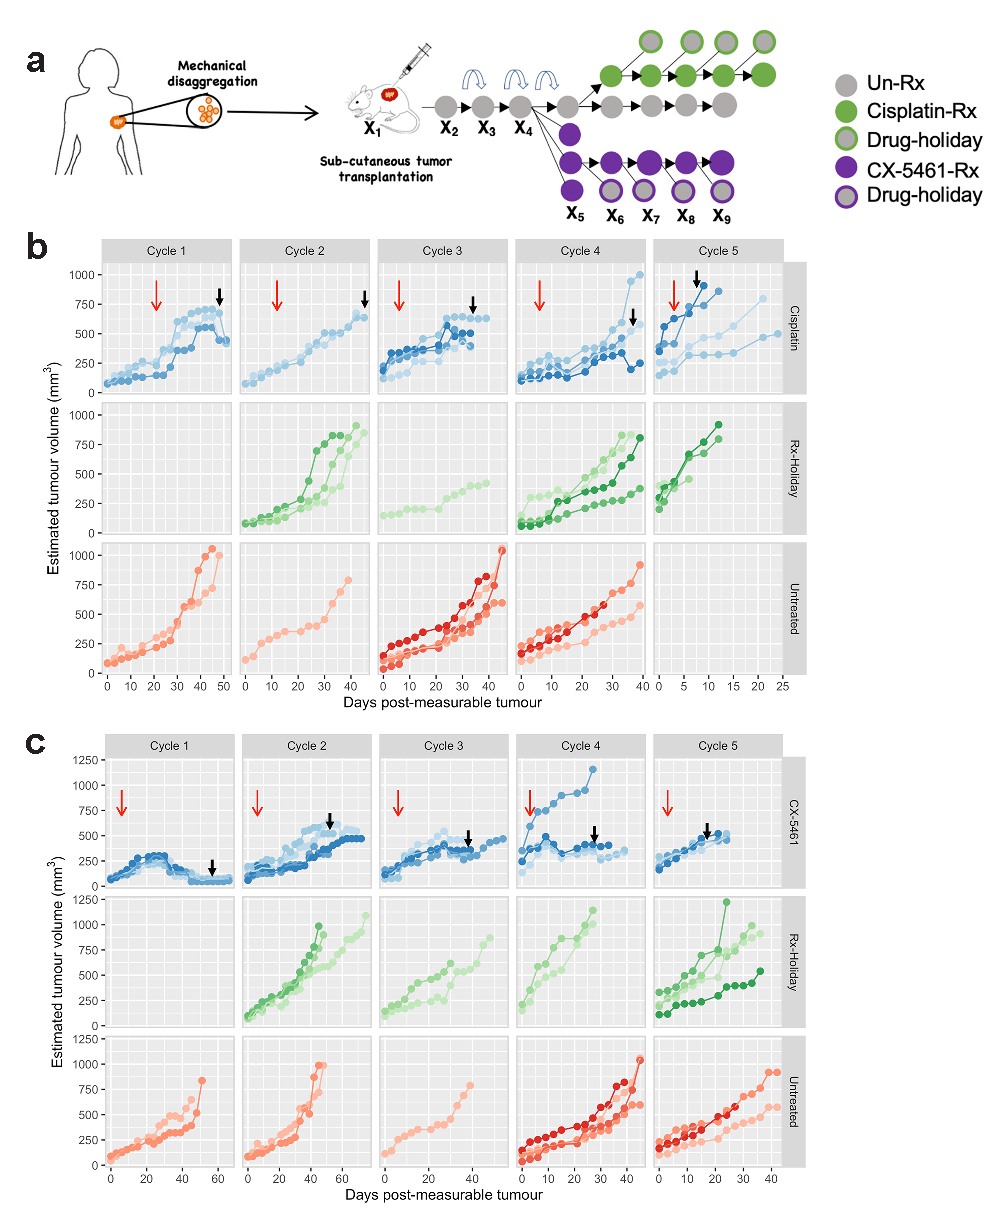
\includegraphics[width=\textwidth]{Figures/chap4/SA535CX5461.png}
	
\caption[SA535 TNBC PDX timeseries with CX-5461]
	{\small
 \textbf{SA535 TNBC PDX timeseries with cisplatin and CX-5461.}
Vertical axis on right indicates the tumor status. The top bar gives cycle numbers and left vertical axis gives tumor measurements. Horizontal axis are days post measurable tumors\textbf{(a)} Experimental overview and passaging details of start and end of cisplatin and CX-5461 treatments. Red arrows point to the start of treatment and black arrows point to the tumor rdigested for sc-WGS.
	   \textbf{(b)} Growth curves of cisplatin treated tumors
	    \textbf{(c)} Growth curves of CX-5461 treated tumors.
	}
	\label{fig:SA535CX5461}
\end{figure}

%..................................................................


\begin{figure}
\centering
\includegraphics[width=\textwidth]{Figures/chap4/SA535combinebarplots.png}
	
\caption[Combined data analysis of SA535 with cisplatin and CX-5461]
	{\small
	\textbf{Combined data analysis of SA535 with cisplatin and CX-5461.}
	   \textbf{(a)} Integer copy number heat map showing vertical columns as chromosomes and each row represent single cell. Red arrows pointing to change in copy number events in that specific clone.
	    \textbf{(b)} Bar plots showing clonal composition at each time point. Vertical axis shows the clonal fraction and horizontal axis presents the passage timepoint.
	     \textbf{(c)} Simplified way to present clonal lineage tree matching the bars composition in \textbf{(a)}.
	}
	\label{fig:SA535combinebarplots}
\end{figure}

%...............................................................

\subsubsection{Drug resistant clones arise from the same precursor}
Integer heat map of copy number heterogeneity was computed using \texttt{sitka} and interestingly cisplatin and CX-5461 treated cells clustered independently from each other and from the un treated cell clusters \textbf{\autoref{fig:SA535combinebarplots} a}. Clonal abundance for the un treated time series depicted increase of Clone Q till passage 7 (X7) but then gradual decrease favouring emerging of clone J in the later generations \textbf{(\autoref{fig:SA535combinebarplots} b (left top panel))}. In cisplatin treated series, clone T showed up expanding under the drug whereas with CX-5461 favored emerging of clone U.
Moreover, the resistant branches having clone S and clone T for cisplatin and clone U for CX-5461, both derive from clone R, which is present early in variable proportions in the two branches, but does not have fitness in the untreated, present but at a very minor proportion. Perhaps its giving an idea that independently, drug resistance has apparently a favored clonal starting point in this PDX \textbf{\autoref{fig:SA535combinebarplots} c}. 

Comparing drug holiday samples from cisplatin and CX-5461 treated time series informed resistant clones are reversible early in the treatment of cisplatin but not in case of CX-5461 \textbf{\autoref{fig:SA535combinebarplots} b (middle and right panels)}
These results require further confirmation by treating more TNBC PDX with CX-5461.



\section{Discussion}
The fitness landscapes are inverted as a result of cisplatin chemotherapy in  triple negative breast cancer PDX models.  We have generated replicate observations in PDX models in two ways: parallel replicate timeseries transplants with cisplatin treatment, and duplicate experiments of specific time points \textbf{\autoref{fig:treatedtimeseriesgreen} a} . In untreated timeseries \textbf{\autoref{fig:SA609barplotanalysis} left panel}, we observe repeated expansion of clone H, relative to lower fitness clones (e.g. clone D). Furthermore, in treated series, we observe the same clonal dynamics - namely that a phylogenetic branch of the population which has low fitness in the untreated control branch is repeatedly observed to selectively expand on treatment.  Notably, we remark in triplicate lines,  highly congruent dynamics with the introduction of treatment between X3 and X4. 

SA609 TNBC drug holiday data suggest the impact of cisplatin selective pressure on the starting tumour cell population is reversible while genomic clonal competition with precursor clones is still possible, but dominates the population once the evolutionary bottleneck narrows and purifies the population.

Furthermore within lines, we observe through duplicate samplings that the clonal expansion patterns are repeatedly observed. With these repeat experiments, we note that the starting population structure is not deterministic of clonal abundance of future population structure.  We attest that while stochastic effects of sampling cannot be ruled out, the monotonic trajectories of clones and repeated observations strongly suggest variation in fitness as a primary determinant. In additional two series other than SA609 TNBC series, we noted that the starting point of treatment experiments harbours a more balanced representation of high and low fitness clones, and therefore are less subject to the sampling bias.  In the last two series, similar inversions of the fitness landscape are observed.  Together, the replicate experiments and addition of 2 new TNBC PDX series indicate that the fitness inversion is not a stochastic effect and establishes with precision that high fitness lineages in the untreated setting are selectively pruned, while low fitness lineages in the untreated setting selectively expand. The observation that drug resistance can have a fitness cost also points to an underlying mechanism of retained sensitivity in early treatment.




